\section{Anhang}
\subsection{Kapazitiver Spannungsteiler}
\label{cap-teiler}

\begin{minipage}[c]{0.4\columnwidth}
    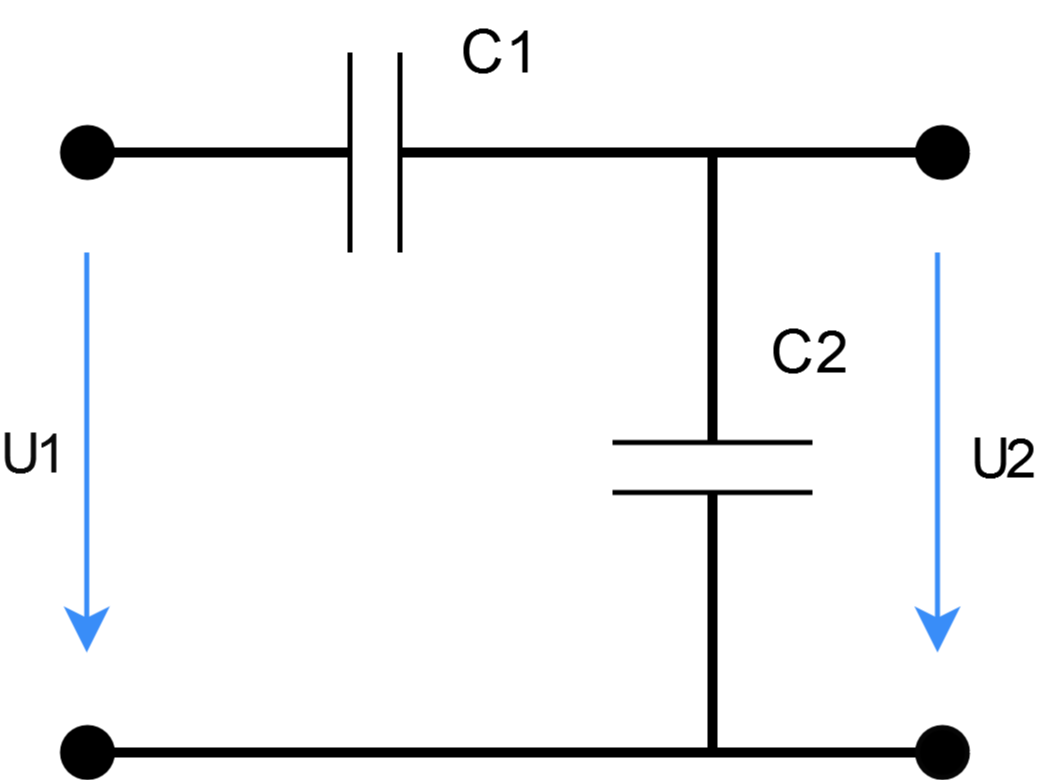
\includegraphics[width=0.7\columnwidth]{images/CapSpannungsteiler.png} 
\end{minipage}
\hfill
\begin{minipage}[c]{0.58\columnwidth}
    $$ \boxed{ U_2 = U_1 \cdot \frac{X_2}{X_1 + X_2} = U_1 \cdot \frac{C_1}{C_1 + C_2} } $$
\end{minipage}

\subsection{Ladung am Kondensator}

\begin{minipage}[c]{0.3\columnwidth}
    $$ \boxed{ Q = C \cdot U } $$
\end{minipage}
\hfill
\begin{minipage}[c]{0.66\columnwidth}
    Knoten isoliert \textrightarrow\ $Q$ bleibt konstant
\end{minipage}

\vspace{0.1cm}

{\small \textrightarrow\ Eine Platte springt um $\Delta V$ \textrightarrow\ andere Platte springt auch um $\Delta V$ ($U_C$ bleibt)} \\
{\small \textrightarrow\ Mit Teiler: $\Delta V_X = \Delta V \cdot \frac{C_1}{C_1 + C_2}$ \ (vgl.\ \ref{cap-teiler})}